
Nella sezione \ref{sec:DervTrasfLorentz} è stato introdotto il concetto di 4-vettore (quadrivettore) tramite il 4-vettore posizione, successivamente si è osservato che è possibile costruire altri 4-vettori, come la 4-velocità, che si trasformano anch'essi con le trasformazioni di Lorentz. Volendo essere più precisi si chiameranno 4-vettori tutti i vettori di $\mathbb{R}^4$ che si trasformano come il 4-vettore posizione.\\ 
La struttura non più euclidea dello spazio-tempo richiede una maggior attenzione nella trattazione dei 4-vettori: è quindi necessario distinguere 4-vettori controvarianti, indicati con $A^{\mu}=(A^0,A^1,A^2,A^3)$, e covarianti, indicati con $A_{\mu}=(A_0,A_1,A_2,A_3)$. I primi si trasformano con le trasformazioni di Lorentz $\Lambda_\nu^\mu$ (\ref{TrasformazioneLorentz}), mentre i secondi con la trasformazione inversa e trasposta, così che utilizzando la convenzione di Einstein\footnote{La convenzione di Einstein è una notazione abbreviata dell'operazione di sommatoria: ogni coppia di indici ripetuti corrisponde ad una sommatoria sottintesa su tale indice. Un esempio può essere: $\sum_k A_{i,k}B^{j,k}= A_{i,k}B^{j,k}$} tali trasformazioni si scrivono:
\begin{equation}
    A'^\mu =\Lambda_\nu^\mu A^\nu \qquad \qquad A_\mu '=(\Lambda^{-1} )^\nu_\mu A_\nu.
\end{equation}
Utilizzando 4-vettori covarianti e controvarianti è possibile ottenere una quantità scalare invariante per le trasformazioni di Lorentz:
\begin{eqnarray*}
    A'^\mu B'_\mu=\Lambda_\alpha^\mu A^\alpha (\Lambda^{-1} )^\beta_\mu B_\beta=A^\alpha \delta_\alpha^\beta B_\beta=A^\alpha B_\alpha
\end{eqnarray*}
dove $ \delta_\alpha^\beta$ è la delta di Kronecker data dal prodotto righe per colonne della matrice della trasformazione di Lorentz con la sua inversa. La quantità appena ottenuta è il prodotto scalare dei 4-vettori $A$ e $B$, questo è esprimibile, come si è visto nella sezione \ref{sec:DervTrasfLorentz}, attraverso l'uso della matrice metrica $g_{\mu \nu}$, questa osservazione consente di trovare una relazione tra componenti controvarianti e covarianti. Fissato un 4-vettore $A_\mu$ allora $\forall B^\nu$: 
\begin{equation}
    B^\mu A_\mu=B^\mu g_{\mu\nu} A^\nu \quad \Rightarrow\quad A_\mu=g_{\mu\nu}A^\nu \ \Leftrightarrow\ A^0=A_0,\ A^i=-A_i \ \ i\in\{1,2,3\}.
\end{equation}
L'operazione algebrica di sommare i prodotti delle componenti di due 4-vettori, come si è fatto nei precedenti calcoli, è nota, secondo la convenzione di Einstien, come contrazione di due indici; come si è visto la contrazione di un indice controvariante con uno covariante da uno scalare Lorentz Invariante.\\

Si consideri ora il 4-vettore posizione $x_\mu$, come si è già visto il luogo dei punti nei quali $x^\mu x_\mu=0$ rappresenta moti che avvengono alla velocità della luce ed è detto cono di luce. In analogia con il 4-vettore posizione ed il cono di luce (Fig. \ref{fig:conoLuce}) è possibile classificare un qualsiasi 4-vettore in base al suo modulo quadro:
\begin{multicols}{2}
    \begin{figure}[H]
        \centering
        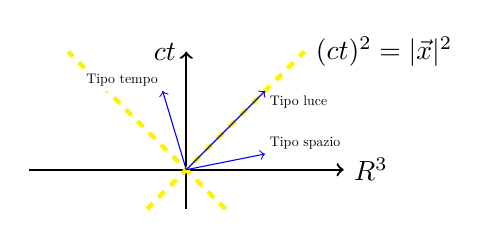
\begin{tikzpicture}
            \draw[->,black,thick] (0,-0.5) -- (0,1.5) node[anchor=east]{$ct$};
            \draw[->,black,thick] (-2,0) -- (2,0) node[anchor=west]{$\mathbb{R}^3$};
            \draw[dashed,yellow,ultra thick] (-0.5,-0.5) -- (1.5,1.5)node[anchor=west, black]{$(ct)^2=|\vec{x}|^2$};
            \draw[dashed,yellow,ultra thick] (0.5,-0.5) -- (-1.5,1.5);
            \draw[->,blue] (0,0) -- (-0.3,1) node[color=black,anchor=south east, scale=.5,fill=white]{Tipo tempo};
            \draw[->,blue] (0,0) -- (1,1) node[color=black,anchor=north west, scale=.5]{Tipo luce};
            \draw[->,blue] (0,0) -- (1,0.2) node[color=black,anchor=south west, scale=.5,fill=white]{Tipo spazio};
        \end{tikzpicture}
        \caption{Cono di luce nel piano}
        \label{fig:conoLuce}
    \end{figure}

    \begin{flalign*}
        A^\mu A_\mu=(A^0)^2-|\vec{A}|^2
        \begin{cases}
            >0\ \ \text{Tipo tempo}\\
            =0\ \ \text{Tipo luce}\\
            <0\ \ \text{Tipo spazio}\\
        \end{cases}
    \end{flalign*}
\vspace*{\fill}
\end{multicols}
Poiché come è già stato anticipato $c$ rappresenta un limite per le velocità allora si può enunciare il seguente principio: \emph{dall'origine di un sistema di riferimento l'informazione non può raggiungere 4-vettori posizione di tipo spazio, ossia al di fuori del cono di luce}.\\

Il concetto di 4-vettore può essere esteso ad oggetti a più indici che si trasformano con le trasformazioni di Lorentz detti 4-tensori, come la matrice metrica o la delta di Kronecker. Anche le componenti di questi oggetti possono essere covarianti o controvarianti, in base a come queste si trasformino, si fa quindi uso della medesima notazioni con indici bassi e alti tenendo conto che però un 4-tensore può avere anche indici misti. Anche nel caso di 4-tensori si può effettuare l'operazione di contrazione di indici, anche tra indici dello stesso tensore: nel caso di contrazione di coppie di indici di cui uno controvariante e uno covariante si ha che la quantità ottenuta è ancora un 4-tensore o uno scalare Lorentz Invariante. \\

Infine si osservi che prendendo un campo scalare $\Phi(t,x,y,z)$ e calcolandone il 4-gradiente $\partial_\mu\Phi=(\frac{1}{c}\frac{\partial\Phi}{\partial t},\frac{\partial\Phi}{\partial x^1},\frac{\partial\Phi}{\partial x^2},\frac{\partial\Phi}{\partial x^3})$ questo risulta essere un 4-vettore in coordinate covarianti, infatti secondo la regola della derivata di funzione composta:
\begin{equation*}
    \partial'_\mu\Phi=\partial_\nu\Phi\ \frac{\partial x^\nu}{\partial x'^\mu}=\partial_\nu\Phi\ (\Lambda^{-1})_\mu^\nu.
\end{equation*}
Analogamente è possibile calcolare la 4-divergenza di un 4-vettore, questa però risulta uno scalare Lorentz invariante infatti:
\begin{equation*}
    \partial'_\mu A'^\mu=\frac{\partial A^\delta}{\partial x^\nu} \frac{\partial x^\nu}{\partial x'^\mu}\Lambda^\mu_\delta=\frac{\partial A^\delta}{\partial x^\nu}(\Lambda^{-1})_\mu^\nu \Lambda^\mu_\delta=\partial_\nu A^\nu=\frac{1}{c}\frac{\partial A^0}{\partial t}+\vnabla\cdot \vec{A}.
\end{equation*} 
Considerazioni di questo tipo possono essere fatte per altri operatori di differenziazione che possono anche agire su 4-tensori risultanti quindi in altri 4-tensori o in scalari, questo poiché sia gli operatori di differenziazione, tramite la regola della derivata di funzione composta, sia i 4-tensori, per definizione, si trasformano con $\Lambda$\footnote{Questa osservazione è valida solamente in relatività speciale dove la trasformazione delle coordinate è lineare, in relatività generale infatti non è più vero che la derivata di un 4-tensore è ancora un 4-tensore o che la 4-divergenza è uno scalare.}. La notazione ad indici alti e bassi diventa quindi utile per evidenziare come si possano costruire quantità tensoriali o scalari invarianti sfruttando quanto appena detto: infatti per esempio la notazione $\partial_\mu A^\mu$ ricorda il prodotto scalare, che come si è visto da luogo ad un invariante di Lorentz come avviene anche per la 4-divergenza.\\
